\section{Motivation}
\begin{frame}{Attention Mechanism}
  \centering
  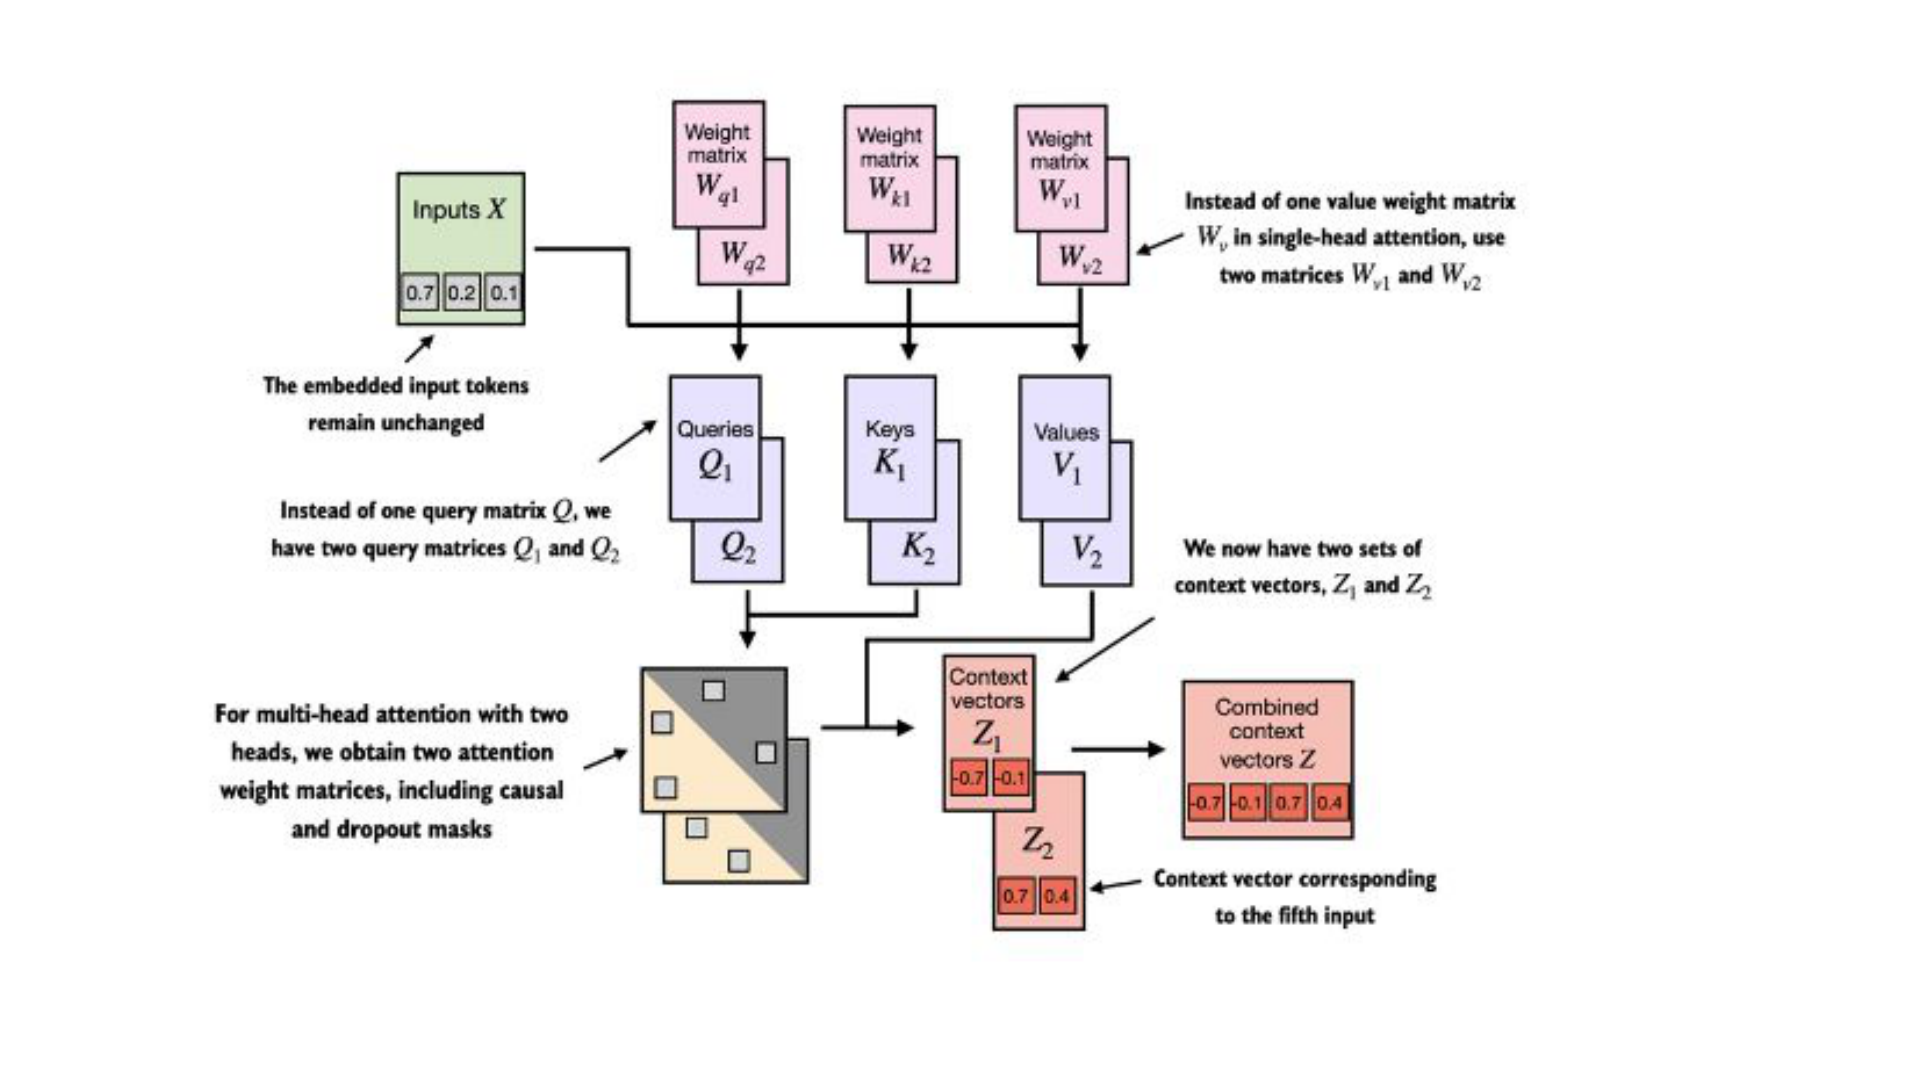
\includegraphics[width=0.8\paperwidth,height=0.62\paperheight,keepaspectratio]{images/attention-deep-dive/attention_multihead_qkv_overview.png}

  {\scriptsize Source: after Sebastian Raschka, \textit{Build a Large Language Model (From Scratch)}, Manning, 2024, Ch.~3 (multi-head attention).}

  {\footnotesize A query is scored against every key, the scores are normalized into weights, and the output is the weighted sum of the values. Running several such heads in parallel gives multi-head attention, covered later.}
\end{frame}


\begin{frame}{Motivation}
  \begin{itemize}
    \item Sequence-to-sequence models struggle with \textbf{long-range dependencies}, making it difficult to capture context over lengthy inputs.
    \item Attention mechanisms address this by allowing the model to \textbf{selectively focus} on relevant parts of the input sequence during processing.
    \item They form the \textbf{backbone} of modern architectures such as \textbf{Transformer models} (e.g., BERT, GPT, ViT).
    \item Attention underpins tasks such as \textbf{translation}, \textbf{summarization}, and \textbf{image captioning}.
  \end{itemize}
  \vspace{1em}
  \textbf{Example:} In machine translation, rather than encoding an entire sentence into a single fixed-size vector, attention enables the model to dynamically focus on relevant source words when generating each target word.
\end{frame}
